\documentclass[usenames,dvipsnames]{beamer}
\usepackage{mycommonstyle}

\title{Bias/Variance and Cross-Validation}
\date{\today}
\author{Nipun Batra and teaching staff}
\institute{IIT Gandhinagar}

\begin{document}
	\maketitle
	
	

	\begin{frame}{A Question!}
What would be the decision boundary of a decision tree classifier? 

\begin{figure}
	\centering
	\includegraphics{../figures/decision-trees/bias-variance-dataset.pdf}
\end{figure}


\end{frame}

\begin{frame}{Decision Boundary for a tree with depth 1}
\begin{figure}%
\centering
\subfloat[Decision Boundary]{{\includegraphics[width=0.45\textwidth]{../figures/decision-trees/bias-variance-depth-1.pdf} }}%
\qquad
\subfloat[Decision Tree]{{\includegraphics[width =0.45\textwidth]{../figures/decision-trees/bias-variance-depth-1-sklearn.pdf} }}%
\label{fig:example}%
\end{figure}
\end{frame}

\begin{frame}{Decision Boundary for a tree with no depth limit}
\begin{figure}%
\centering
\subfloat[Decision Boundary]{{\includegraphics[width=0.42\textwidth]{../figures/decision-trees/bias-variance-full-depth.pdf} }}%
\qquad
\subfloat[Decision Tree]{{\includegraphics[width =0.3\textwidth]{../figures/decision-trees/bias-variance-full-depth-sklearn.pdf} }}%
\label{fig:example}%
\end{figure}
\end{frame}


\begin{frame}{Are deeper trees always better?}
\only<1-2>{
As we saw, deeper trees learn more complex decision boundaries.
}

\only<2>{
\vspace{1cm}
But, sometimes this can lead to $poor$ $generalization$
}	
\end{frame}

\begin{frame}{An example}
Consider the dataset below
\begin{figure}%
\centering
\subfloat[Train Set]{{\includegraphics[width=0.45\textwidth]{../figures/decision-trees/bias-variance-dataset-2.pdf} }}%
\qquad
\subfloat[Test Set]{{\includegraphics[width =0.45\textwidth]{../figures/decision-trees/bias-variance-dataset-2-test.pdf} }}%
\label{fig:example}%
\end{figure}
\end{frame}

\begin{frame}{Underfitting}
Underfitting is also known as $high$ $bias$, since it has a very biased incorrect assumption.
\begin{figure}%
\centering
\subfloat[Decision Boundary]{{\includegraphics[width=0.45\textwidth]{../figures/decision-trees/bias-variance-depth-2.pdf} }}%
\qquad
\subfloat[Decision Tree]{{\includegraphics[width =0.45\textwidth]{../figures/decision-trees/bias-variance-depth-2-sklearn.pdf} }}%
\label{fig:example}%
\end{figure}
\end{frame}

\begin{frame}{Overfitting}
Overfitting is also known as $high$ $variance$, since very small changes in data can lead to very different models.\\
Decision tree learned has depth of 10.
\begin{center}
\includegraphics[scale=0.5]{../figures/decision-trees/bias-variance-full-depth.pdf}
\end{center}
\end{frame}


\begin{frame}{Intution for Variance}
A small change in data can lead to very different models.\\
\vspace{1cm}
\begin{columns}
\begin{column}{0.5\textwidth}{\hspace{1.75cm} Dataset 1}
\begin{center}
\includegraphics[width = \textwidth]{../figures/decision-trees/bias-variance-dataset-2.pdf}
\end{center}
\end{column}
\begin{column}{0.5\textwidth}{\hspace{1.75cm} Dataset 2}
\begin{center}
\includegraphics[width = \textwidth]{../figures/decision-trees/bias-variance-dataset-2-2.pdf}
\end{center}
\end{column}
\end{columns}
\end{frame}


\begin{frame}{Intution for Variance}
\begin{columns}
\begin{column}{0.5\textwidth}
\begin{center}
\includegraphics[scale=0.2]{../figures/decision-trees/bias-variance-full-depth-sklearn.pdf}
\end{center}
\end{column}
\begin{column}{0.5\textwidth}
\begin{center}
\includegraphics[scale=0.2]{../figures/decision-trees/bias-variance-full-depth-2-sklearn.pdf}
\end{center}
\end{column}
\end{columns}
\end{frame}


\begin{frame}{A Good Fit}
\begin{columns}
\begin{column}{0.5\textwidth}
\includegraphics[width=\textwidth]{../figures/decision-trees/bias-variance-good-fit.pdf}
\end{column}
\begin{column}{0.5\textwidth}
\includegraphics[width =\textwidth]{../figures/decision-trees/bias-variance-good-fit-sklearn.pdf}
\end{column}
\end{columns}

\end{frame}

\begin{frame}{Accuracy vs Depth Curve}
\begin{center}
\includegraphics[scale=0.55]{../figures/decision-trees/bias-variance-accuracy-vs-depth.pdf}
\end{center}
\pause As depth increases, train accuracy improves\\
\pause As depth increases, test accuracy improves till a point\\
\pause At very high depths, test accuracy is not good (overfitting). 

\end{frame}

\begin{frame}{Accuracy vs Depth Curve : Underfitting}
The highlighted region is the underfitting region.\\
Model is too simple (less depth) to learn from the data. 
\begin{center}
\includegraphics{../figures/decision-trees/bias-variance-accuracy-vs-depth-underfitting.pdf}
\end{center}
\end{frame}

\begin{frame}{Accuracy vs Depth Curve : Overfitting}
The highlighted region is the overfitting region.\\
Model is complex (high depth) and hence also learns the anomalies in data. 
\begin{center}
\includegraphics{../figures/decision-trees/bias-variance-accuracy-vs-depth-overfitting.pdf}
\end{center}
\end{frame}

\begin{frame}{Accuracy vs Depth Curve }
The highlighted region is the good fit region.\\
We want to maximize test accuracy while being in this region.
\begin{center}
\includegraphics{../figures/decision-trees/bias-variance-accuracy-vs-depth-good-fit.pdf}
\end{center}
\end{frame}

\begin{frame}{The big question!?}
\only<1-2>{
How to find the optimal depth for a decision tree?\\
}
\only<2>{
\vspace{1cm}
Use cross-validation!
}
\end{frame}


\begin{frame}{Our General Training Flow}
\includegraphics[width = \textwidth]{../diagrams/cross-validation/general-workflow}
\end{frame}

\begin{frame}{K-Fold cross-validation: Utilise full dataset for testing}
\includegraphics[width = \textwidth]{../diagrams/cross-validation/cross-validation-train-test}
\end{frame}

\begin{frame}{The Validation Set}
\includegraphics[width = \textwidth]{../diagrams/cross-validation/validation-workflow}
\end{frame}

\begin{frame}{Nested Cross Validation}
Divide your training set into $K$ equal 	parts.\\
Cyclically use 1 part as ``validation set" and the rest for training.\\
\begin{center}
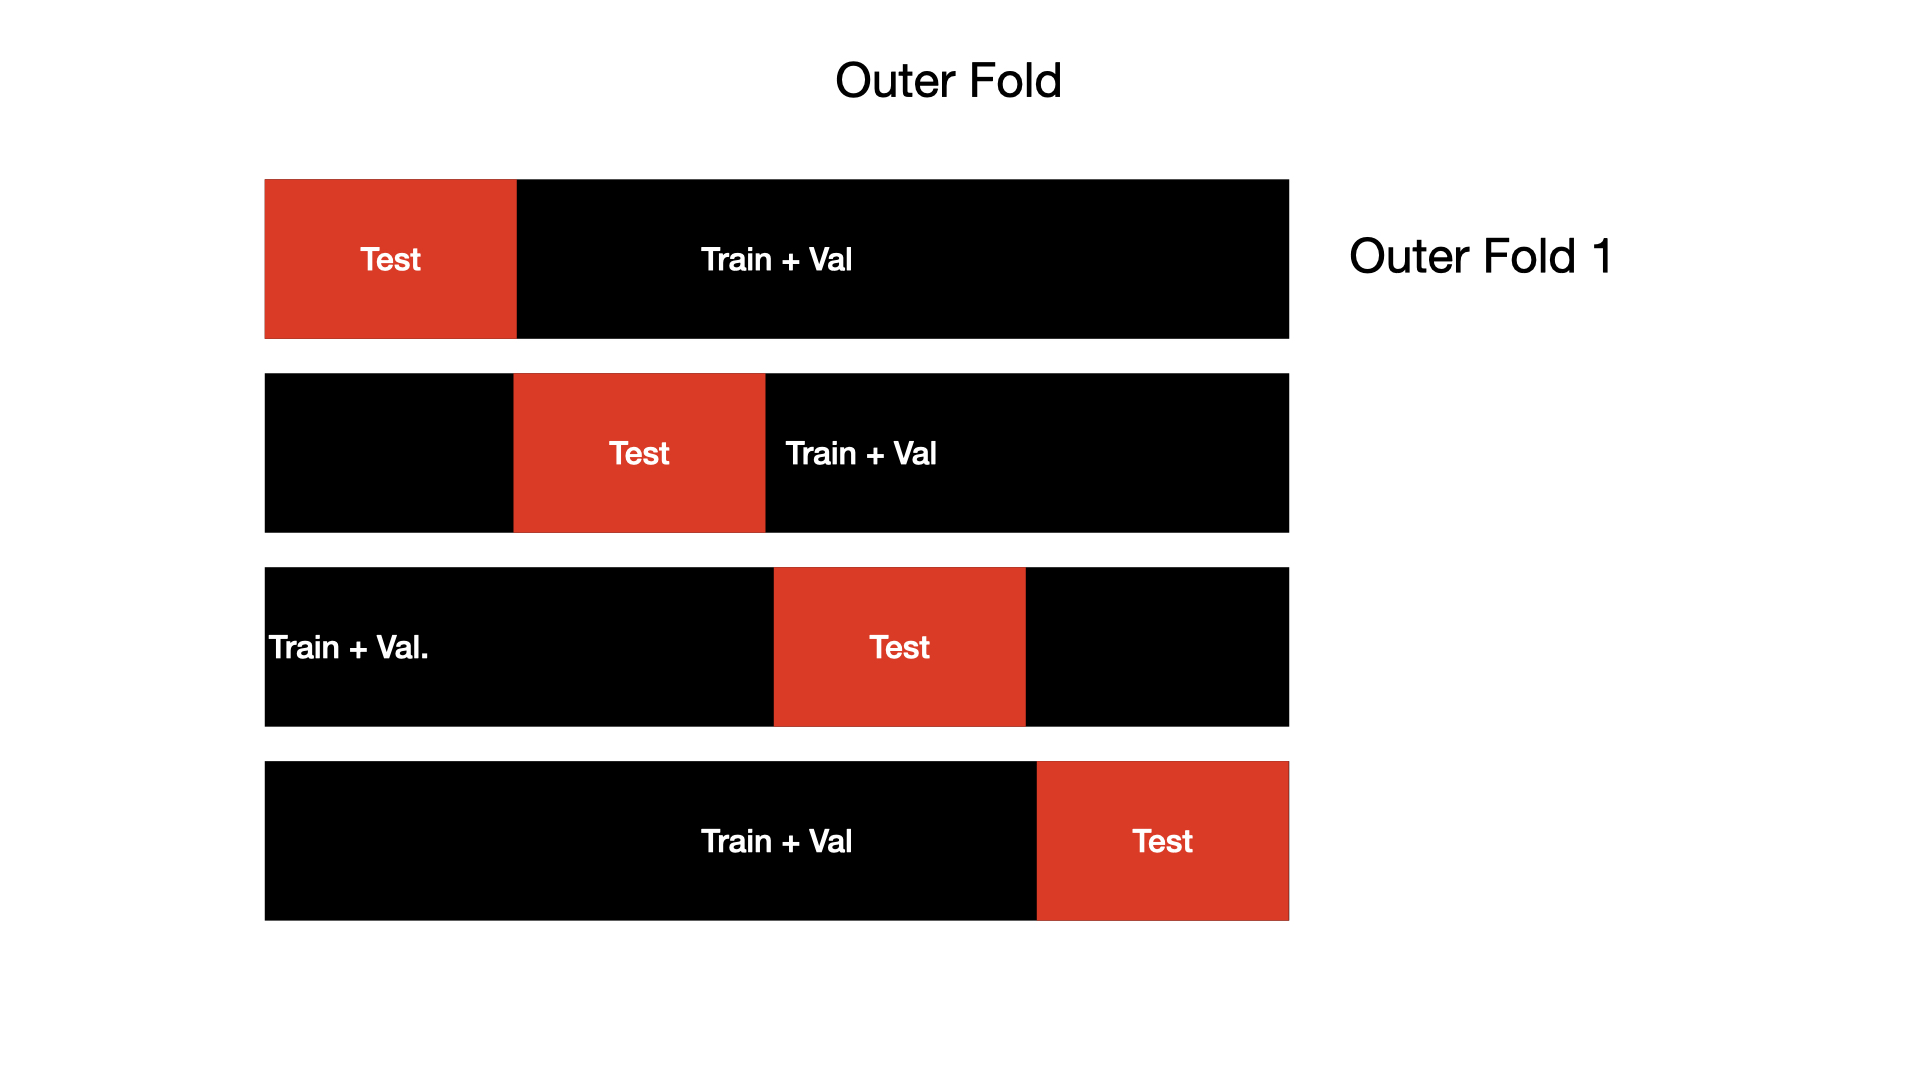
\includegraphics[scale=0.18]{./cross-validation/cross-validation.001.jpeg}
\end{center}
\end{frame}

\begin{frame}{Nested Cross Validation}
	Divide your training set into $K$ equal 	parts.\\
	Cyclically use 1 part as ``validation set" and the rest for training.\\
	\begin{center}
	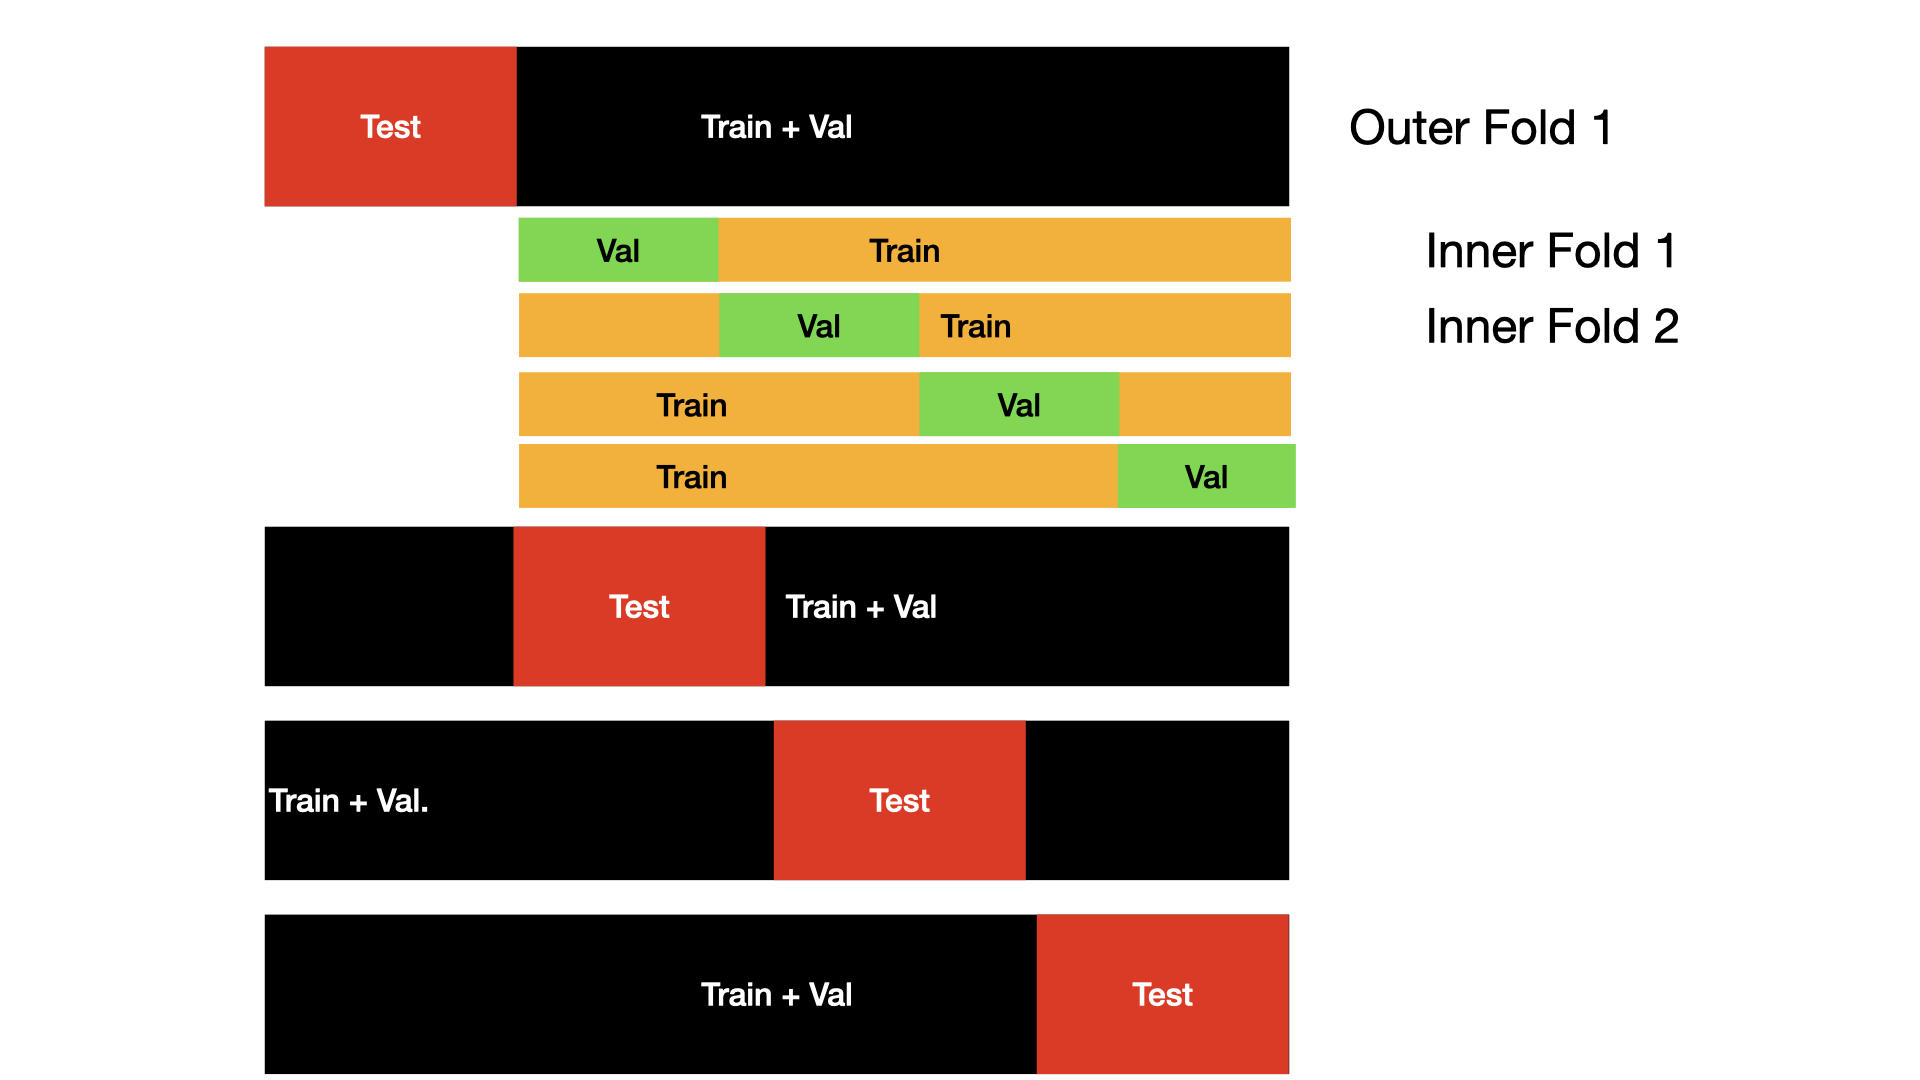
\includegraphics[scale=0.18]{./cross-validation/cross-validation.002.jpeg}
	\end{center}
	\end{frame}
	


\begin{frame}{Next time: Ensemble Learning}
\begin{itemize}
\item How to combine various models?
\item Why to combine multiple models?
\item How can we reduce bias?
\item How can we reduce variance?
\end{itemize}
\end{frame}

\end{document}